% Standardinkluderingsfil
%
%  untitled
%
%  Created by David Granqvist on 2008-09-08.
%  Modified by Martin Erola
%

% Set document format/class
\documentclass[a4paper,twoside]{article}

%%%%%%%%%%%%%%%%%%%
% Include packages
%
\usepackage[utf8]{inputenc}   % Use utf-8 encoding for foreign characters
\usepackage[swedish]{babel}   % Support for swedish letters
\usepackage{fullpage}         % Setup for fullpage use
\usepackage{fancyhdr}         % Running Headers and footers
\usepackage{boxedminipage}    % Surround parts of graphics with box
\usepackage{listings}         % Package for including code in the document
\usepackage{ifpdf}            % Recommended way for checking for PDFLaTeX:
\usepackage{tabularx}         % Tabeller med automatisk stretch
% \usepackage[nofancy]{svninfo} % Extract Subversion info about the file
% \usepackage{color}          % Color
% \usepackage{lastpage}       % Total page count

% Graphics
\ifpdf
\usepackage[pdftex]{graphicx}
\else
\usepackage{graphicx}
\fi

%%%%%%%%%%%%%%%%%%%%%%%%%%%%%%%%%%%%%%%%%%%%%%%%%%%%%%%%%%
% Uncomment some of the following if you use the features
%

% Multipart figures
%\usepackage{subfigure}

% More symbols
%\usepackage{amsmath}
%\usepackage{amssymb}
%\usepackage{latexsym}

% If you want to generate a toc for each chapter (use with book)
% \usepackage{minitoc}

%%%%%%%%%%%%%%%%%%%%
% Document settings
%

% Header
\pagestyle{fancy}
% Sätter en marginal mellan header och (ovanstående?) text %
\setlength\headsep{10pt}
% Sätter höjden på headern
\setlength{\headheight}{32pt}

% Sätter styckesinställningar
\setlength\parindent{0pt}
\setlength\parskip{10pt}



\ifpdf
  \DeclareGraphicsExtensions{.pdf, .jpg, .tif, .png}
  \pdfinfo{            
    /Title  (Use-case model)
    /Author (PUM-grupp 1)
  }
\else
  \DeclareGraphicsExtensions{.eps, .jpg}
\fi

\title{Use-case model}
\author{PUM-grupp 1}
\date{\today}

\begin{document}

\maketitle\thispagestyle{empty}
\newpage

{\centering \Large{Dokumenthistorik\\}}

\vspace{10pt}
\begin{tabularx}{\textwidth}{ |l|l|X|l|l| }
  \hline
    \textbf{version} & \textbf{datum} & \textbf{utförda ändringar} & \textbf{utförda av} & \textbf{granskad} \\
	\hline 
  1.0 & 2009-02-12 &  Första versionen klar för inlämning  & Alla & Alla   \\
  \hline
\end{tabularx}

\newpage
\setcounter{tocdepth}{2}
\tableofcontents
\newpage

\section{Inledning}
För att enklare förstå de olika användarfallen vi identifierat och skapa en överblick över dem har vi gjort en användarfalls model där vi grafisk visar hur användare och system hänger ihop.
\section{Överblick}
%Skapa en överblick för systemet, dvs beskriv vad systemet gör och vad desss mål är.
Systemet i fråga är ett distribuerat versionshanteringssystem. Meningen med detta system är att man på ett enkelt sätt ska kunna hantera dokument i en wiki-miljö samtidigt som man inte ens behöver vara uppkopplad. När användaren sedan kopplar upp sig mot internet kan denne synkronisera sina ändringar med andra användares ändringar.
\section{Användarfalls diagram}
 \begin{figure}[H] %  figure placement: here, top, bottom, or page
  \centering
  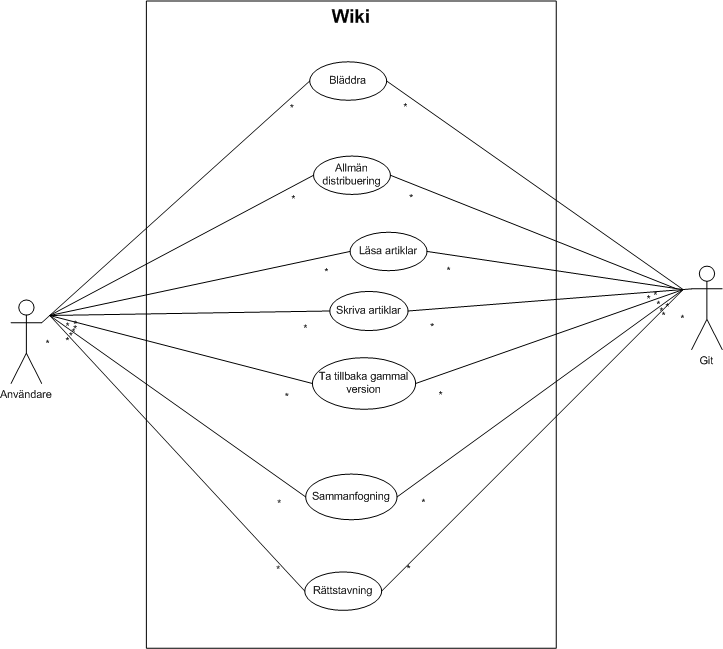
\includegraphics[scale=0.50]{Use-case-diagram.png}
\end{figure}
%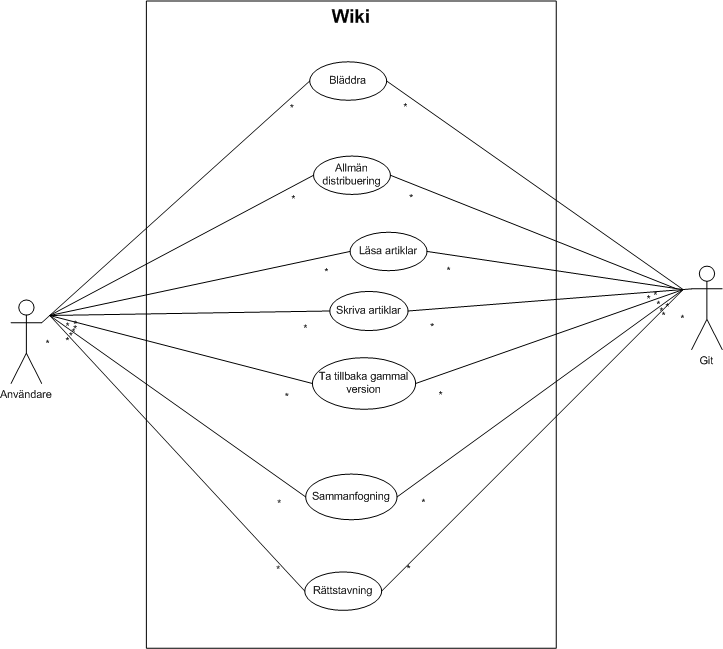
\includegraphics{Use-case-diagram.png}
\section{Aktörer}
%Beskriv alla aktörer som finns med i use-case diagrammet.
\begin{itemize}
	\item Lokal användare
	\\Denna aktör representerar en normal användare som sitter vid sin dator och ej är uppkopplad mot internet.
	\item Extern användare
	\\Denna aktör representerar en användare som sitter uppkopplad mot systemet och internet.
\end{itemize}
\section{Användarfall}
%Rada upp de olika use-cases som finns.
\subsection{Bläddra}
Detta användarfall beskriver hur man bläddrar bland dokument.
\subsection{Läsa artiklar}
Detta användarfall beskriver hur man läser sina egna eller andra användares artiklar.
\subsection{Skriva en artikel}
Detta användarfall beskriver hur man skriver en artikel.
\subsection{Ta tillbaka gammal version}
Detta användarfall beskriver hur man tar tillbaka en gammal version av en fil.
\subsection{Sammanslagning}
Detta användarfall beskriver hur man sammanfogar två eller flera filer med varandra.
\subsection{Rättstavning}
Detta användarfall beskriver hur man kan använda rättstavningskontrollen.
\end{document}
